%NEURAL PRESY ;)

%----------------------------------------------------------------------------------------
%   PACKAGES AND THEMES
%----------------------------------------------------------------------------------------

\documentclass{beamer}

\mode<presentation> {

% The Beamer class comes with a number of default slide themes
% which change the colors and layouts of slides. Below this is a list
% of all the themes, uncomment each in turn to see what they look like.

%\usetheme{default}
%\usetheme{AnnArbor}
%\usetheme{Antibes}
%\usetheme{Bergen}
\usetheme{Berkeley}
%\usetheme{Berlin}
%\usetheme{Boadilla}
%\usetheme{CambridgeUS}
%\usetheme{Copenhagen}
%\usetheme{Darmstadt}
%\usetheme{Dresden}
%\usetheme{Frankfurt}
%\usetheme{Goettingen}
%\usetheme{Hannover}
%\usetheme{Ilmenau}
%\usetheme{JuanLesPins}
%\usetheme{Luebeck}
%\usetheme{Madrid}
%\usetheme{Malmoe}
%\usetheme{Marburg}
%\usetheme{Montpellier}
%\usetheme{PaloAlto}
%\usetheme{Pittsburgh}
%\usetheme{Rochester}
%\usetheme{Singapore}
%\usetheme{Szeged}
%\usetheme{Warsaw}

% As well as themes, the Beamer class has a number of color themes
% for any slide theme. Uncomment each of these in turn to see how it
% changes the colors of your current slide theme.

%\usecolortheme{albatross}
%\usecolortheme{beaver}
%\usecolortheme{beetle}
%\usecolortheme{crane}
%\usecolortheme{dolphin}
%\usecolortheme{dove}
%\usecolortheme{fly}
%\usecolortheme{lily}
%\usecolortheme{orchid}
%\usecolortheme{rose}
%\usecolortheme{seagull}
%\usecolortheme{seahorse}
%\usecolortheme{whale}
%\usecolortheme{wolverine}

%\setbeamertemplate{footline} % To remove the footer line in all slides uncomment this line
%\setbeamertemplate{footline}[page number] % To replace the footer line in all slides with a simple slide count uncomment this line

\setbeamertemplate{navigation symbols}{} % To remove the navigation symbols from the bottom of all slides uncomment this line
}

\usepackage{graphicx} % Allows including images
\usepackage{booktabs} % Allows the use of \toprule, \midrule and \bottomrule in tables
\usepackage{caption}
\usepackage{subcaption}
\usepackage{algorithm,algorithmic}

% tikz and associated macros
\usepackage{tikz}
\usepackage{tikz-cd}

\usepackage{pgfplots}
\def\layersep{2cm}
\def\nodesep{0.25cm}
\newcommand*{\Scale}[2][4]{\scalebox{#1}{$#2$}}%
\newcommand*{\Resize}[2]{\resizebox{#1}{!}{$#2$}}%
\newcommand\sep{1.9cm}
\newcommand\height{0.9cm}
\usetikzlibrary{decorations.pathmorphing, backgrounds}
\tikzset{snake it/.style={decorate, decoration=snake}}

%
%

% math
\usepackage{amsthm}
\usepackage{amsmath}
\usepackage{amssymb}
\usepackage{mathabx}

\numberwithin{equation}{subsection}
\numberwithin{theorem}{subsection}

\DeclareSymbolFont{cmlargesymbols}{OMX}{cmex}{m}{n}
\let\sumop\relax
\DeclareMathSymbol{\sumop}{\mathop}{cmlargesymbols}{"50}


\def\reals{{\mathbb R}}
\def\torus{{\mathbb T}}
\def\integers{{\mathbb Z}}
\def\rationals{{\mathbb Q}}
\def\expect{\mathop{{\mathbb{E}}}}
\def\tens{\mathop{{\bigotimes}}}
\def\naturals{{\mathbb N}}
\def\complex{{\mathbb C}\/}
\def\distance{\operatorname{distance}\,}
\def\support{\operatorname{support}\,}
\def\dist{\operatorname{dist}\,}
\def\Span{\operatorname{span}\,}
\def\degree{\operatorname{degree}\,}
\def\kernel{\operatorname{kernel}\,}
\def\dim{\operatorname{dim}\,}
\def\codim{\operatorname{codim}}
\def\trace{\operatorname{trace\,}}
\def\dimension{\operatorname{dimension}\,}
\def\codimension{\operatorname{codimension}\,}
\def\kernel{\operatorname{Ker}}
\def\Re{\operatorname{Re\,} }
\def\Im{\operatorname{Im\,} }
\def\eps{\varepsilon}
\def\lt{L^2}
\def\bull{$\bullet$\ }
\def\det{\operatorname{det}}
\def\Det{\operatorname{Det}}
\def\diameter{\operatorname{diameter}}
\def\symdif{\,\Delta\,}
\newcommand{\norm}[1]{ \|  #1 \|}
\newcommand{\set}[1]{ \left\{ #1 \right\} }
\def\suchthat{\mathrel{}\middle|\mathrel{}}
\def\one{{\mathbf 1}}
\def\cl{\text{cl}}

\def\newbull{\medskip\noindent $\bullet$\ }
\def\nobull{\noindent$\bullet$\ }
\def\defeq{\stackrel{\text{def}}{=}}


\def\scriptf{{\mathcal F}}
\def\scriptq{{\mathcal Q}}
\def\scriptg{{\mathcal G}}
\def\scriptm{{\mathcal M}}
\def\scriptb{{\mathcal B}}
\def\scriptc{{\mathcal C}}
\def\scriptt{{\mathcal T}}
\def\scripti{{\mathcal I}}
\def\scripte{{\mathcal E}}
\def\scriptv{{\mathcal V}}
\def\scriptw{{\mathcal W}}
\def\scriptu{{\mathcal U}}
\def\scriptS{{\mathcal S}}
\def\scripta{{\mathcal A}}
\def\scriptr{{\mathcal R}}
\def\scripto{{\mathcal O}}
\def\scripth{{\mathcal H}}
\def\scriptd{{\mathcal D}}
\def\scriptl{{\mathcal L}}
\def\scriptn{{\mathcal N}}
\def\scriptp{{\mathcal P}}
\def\scriptk{{\mathcal K}}
\def\scriptP{{\mathcal P}}
\def\scriptj{{\mathcal J}}
\def\scriptz{{\mathcal Z}}
\def\scripts{{\mathcal S}}
\def\scriptx{{\mathcal X}}
\def\scripty{{\mathcal Y}}
\def\frakv{{\mathfrak V}}
\def\frakG{{\mathfrak G}}
\def\frakB{{\mathfrak B}}
\def\frakC{{\mathfrak C}}



%----------------------------------------------------------------------------------------
%   TITLE PAGE
%----------------------------------------------------------------------------------------

\title[OpenBrain]{OpenBrain: Backpropagation Free RL}

\author[Guss \& Zhong et. al]{
\includegraphics[height=2cm,width=2cm]{BlueGold_fill_small.png}\\   Guss,  Zhong  \\ Kuznetsov,  \ Kumar,  Golmant, Johansen,  Bartlett}
\date{April 22, 2016} % Date, can be changed to a custom date
\makeatletter
\newcommand{\verbatimfont}[1]{\renewcommand{\verbatim@font}{\ttfamily#1}}
\makeatother
\begin{document}

\begin{frame}
\titlepage
\end{frame}

\addtobeamertemplate{frametitle}{}{%
\begin{tikzpicture}[remember picture,overlay]
\node[anchor=north east,yshift=10pt] at (current page.north east) {
\includegraphics[height=2cm]{White_outline_small_name_transparent.png}};
\end{tikzpicture}}

\begin{frame}

\begin{center}
\Huge
\end{center}


\frametitle{Overview}
\tableofcontents
\end{frame}

\begin{frame}
\frametitle{The Problem}
    \Huge{\centerline{Can we decentralize }}
    \Huge{\centerline{deep reinforcement learning?}}
\end{frame}

\begin{frame}
\frametitle{The Problem}
    \Huge{\centerline{Can we decentralize }}
    \Huge{\centerline{deep reinforcement learning?}}
    \Huge{\centerline{\textbf{Yes.} Here's how. }}
\end{frame}


%----------------------------------------------------------------------------------------
%   PRESENTATION SLIDES
%----------------------------------------------------------------------------------------
\section{Background}
\begin{frame}[fragile]
  \frametitle{Background on Reinforcement Learning}
  \textbf{The setup.}
  \begin{enumerate}
    \item Environment, $E = (\mathcal{S}, \mathcal{A}, \mathcal{R}, \rho, r)$.
    \begin{enumerate}
    \item State space, $\mathcal{S} = \mathbb{R}^n$
    \item Action space, $\mathcal{A} = \mathbb{R}^m$
    \item Reward space, $\mathcal{R} = \mathbb{R}$
    \item Transition function, $\rho(s'\ |\ s,a)$. Given a previous state $s$ and action $a$, environment gives $s'$.
    \item Reward function $r(s,a) \in \mathcal{R}$.
    \end{enumerate}
    \item Deterministic agent $\pi: \mathcal{S} \to \mathcal{A}$ acts in $E$.
    \begin{equation*}
      \begin{tikzcd}
          s_1 \arrow{r}{\pi} & a_1 \arrow{r}{\rho, r} & s_2, r_2 \arrow{r}{\pi}& a_2  \arrow{r}{\rho, r} & \cdots
         \end{tikzcd}
    \end{equation*}
    Eg. Pacman sees the screen, and decides to move $\uparrow, \downarrow, \rightarrow, \leftarrow$ and then gets a reward for eating food.
  \end{enumerate}
\end{frame}
\begin{frame}
\frametitle{Background on Reinforcement Learning}
  \begin{center}
    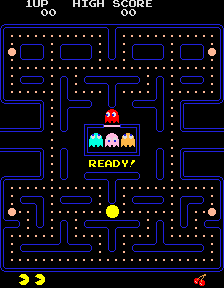
\includegraphics[width=0.5\textwidth]{Pac-man.png}
  \end{center}
\end{frame}

\begin{frame}
\frametitle{Background on Reinforcement Learning}
  \textbf{The action-value function (simplified).}
  \begin{enumerate}
    \item  The future expected reward of an agent $\pi$ is
    \begin{equation*}
      Q^\pi(s_t, a_t) = \underbrace{r(s_t, a_t)}_{\text{reward for } a_t} + \sum_{n={t+1}}^\infty \gamma^n r(s_n, \pi(s_n))
    \end{equation*}
    \item The Bellman equation gives us
    \begin{equation*}
      Q^\pi(s_t, a_t) = r_t + \gamma Q^\pi(s_{t+1}, \pi(s_{t+1}))
    \end{equation*}`'
    \item Given some state $s_t$, the \textbf{best} agent, $\pi^*$ is one that take action
    \begin{equation*}
      a_t = \arg \max_a Q(s_t, a).
    \end{equation*}
  \end{enumerate}
\end{frame}

\begin{frame}
\frametitle{Background on Reinforcement Learning}
  \textbf{The action-value function (simplified).}
  \begin{enumerate}
    \item The $Q$ function for $\pi^*$ is
    \begin{equation*}
      Q^*(s_t, a_t) = r_t + \gamma \arg \max_a Q^\pi(s_{t+1}, a).
    \end{equation*}
    \item We can \emph{approximate} this with deep learning!
    \begin{enumerate}
      \item Make a neural network $\scriptn: \scripts \to \mathbb{R}^n$ which predicts
      the future reward of taking each possible action
      \begin{equation*}
        \scriptn(s_t) =\begin{pmatrix}
            Q^*(s_t, a_1) \\
             Q^*(s_t, a_2)\\
             \vdots \\
              Q^*(s_t, a_n)
        \end{pmatrix}
      \end{equation*}
    \end{enumerate}
  \end{enumerate}
\end{frame}

\begin{frame}
\frametitle{Background on Reinforcement Learning}
  \textbf{Deep Q-Learning}
\begin{center}
  \begin{tikzpicture}
\bode[rectangle] at (0,0) (A) {$s_t$};
\node[rectangle] at (1.5,0) [draw,thick,minimum width=1cm,minimum height=2cm] (B) {$\scriptn$};
\node[rectangle] at (4.4, 2)  [draw, fill=red!30] (C1) {$Q^*(s_t,a_1) = -12$};
\node[rectangle] at (4.4, 1)  [draw, fill=red!30] (C2) {$Q^*(s_t,a_2) = 0.17$};
\node[rectangle] at (4.4, 0)  [draw, fill=green!30] (C3) {$Q^*(s_t,a_3) = 0.22$};
\node[rectangle] at (4.4, -1) [draw, fill=red!30]  (C4) {$Q^*(s_t,a_4) = 0.03$};
\node[rectangle] at (4.4, -2) [draw, fill=red!30]  (C5) {$Q^*(s_t,a_5) = -3.2$};
\node[rectangle] at (8.2, 0) (D) {$ \pi(s_t) =  \arg \max_a \scriptn(s_t)$};
\draw[->] (A) edge (B);
\draw[->] (B) edge (C1.west);
\draw[->] (B) edge (C2.west);
\draw[->] (B) edge (C3.west);
\draw[->] (B) edge (C4.west);
\draw[->] (B) edge (C5.west);
\end{tikzpicture}
\end{center}
\end{frame}

\begin{frame}
    \Huge{\centerline{Can we do better?}}
\end{frame}

\begin{frame}
  \frametitle{Background on Reinforcement Learning}
  \textbf{Deep Determisitic Policy Gradient}
  \begin{enumerate}
    \item Actor neural network $\mu: \scripts \to \scripta$
    \item Critic network $Q^\mu: \scripts \times \scripta \to \mathbb{R}$
    \item Performance of $\mu$ is $Q^\mu(s_t, \mu(s_t))$. \textbf{Maximize performance!} $\nabla_W Q^{\mu}(s_t, a_t) = \nabla_a Q^\mu(s_t,a) \cdot \nabla_W \mu(s_t)$
  \end{enumerate}
\begin{center}
  \begin{tikzpicture}
\bode[rectangle] at (0,0) (A) {$s_t$};
\node[rectangle] at (1.75,0) [draw,thick,minimum width=0.2cm,minimum height=1.8cm, fill=black] (BC1) {};
\node[rectangle] at (2.25,0) [draw,thick,minimum width=0.2cm,minimum height=1.8cm, fill=black] (BC2) {};
\node[rectangle] at (1.5,0) [draw,thick,minimum width=0.3cm,minimum height=2cm] (B1) {};
\node[rectangle] at (2,0) [draw,thick,minimum width=0.3cm,minimum height=2cm] (B2) {};
\node[rectangle] at (2.5,0) [draw,thick,minimum width=0.3cm,minimum height=2cm] (B3) {};
\node[rectangle] at (3.5,0) (action) {$a_t$};
\draw[->] (B3.east) edge (action.west);
\draw[brace] (B1.north) -- node [position label,yshift=2ex] {$\mu$} (B3.north);
\draw[->] (A) edge (B1);

\node[rectangle] at (2.7+ 1.75,-1.5) [draw,thick,minimum width=0.2cm,minimum height=1.8cm, fill=black] (QC1) {};
\node[rectangle] at (2.7+ 2.25,-1.5) [draw,thick,minimum width=0.2cm,minimum height=1.8cm, fill=black] (QC2) {};
\node[rectangle] at (2.7+ 1.5,-1.5) [draw,thick,minimum width=0.3cm,minimum height=2cm] (Q1) {};
\node[rectangle] at (2.7+ 2,-1.5) [draw,thick,minimum width=0.3cm,minimum height=2cm] (Q2) {};
\node[rectangle] at (2.7+ 2.5,-1.5) [draw,thick,minimum width=0.3cm,minimum height=2cm] (Q3) {};
\draw[brace] (Q1.north) -- node [position label,yshift=2ex] {$Q^\mu$} (Q3.north);
\draw[->, bend right] (A) edge (Q1.west);
\draw[->, bend right] (action) edge (Q1.west);
\node[rectangle] at (2.7+ 4,-1.5) (critic) {$Q^{\mu}(s_t, a_t)$};
\draw[->] (Q3.east) edge (critic.west);
\end{tikzpicture}
\end{center}
\end{frame}


%------------------------------------------------
\section{Our Approach} % Sections can be created in order to organize your presentation into discrete blocks, all sections and subsections are automatically printed in the table of contents as an overview of the talk
%---------------- -------------------------------
\begin{frame}
  \frametitle{Our Approach}
      \begin{columns}
      \begin{column}{0.6\textwidth}

  \textbf{Neuromorphically Local Agents}
  \begin{enumerate}

    \item Every neuron in the brain is an agent!
    \item Anterior neurons are the state that $\mu^n$ sees.
    \item The action of each $\mu^n$ is its output:
    \begin{equation*}
      \mu^n(s_t) = \sigma\left(\sum_{i=1}^m W_{in}s_t^{(i)}   \right) = a_t
    \end{equation*}
  \end{enumerate}
      \end{column}
      \begin{column}{0.4\textwidth}
      \begin{figure}
          \begin{centering}
            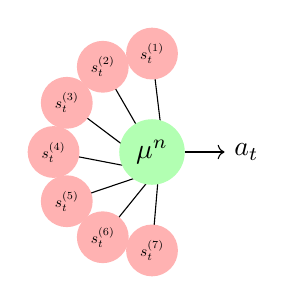
\begin{tikzpicture}
              \foreach \a in {1,2,...,7}{
              \path[draw, ->] (\a*360/6: 0.25cm)  -- (\a*360/12 + 60: 1.5cm-0.25cm) node[circle, fill=red!30, scale=0.8] {$\Scale[0.7]{s_t^{(\a)}}$};

              }
            \node[circle, style=dashed, fill=green!30] (A) {$\mu^n$};
            \node[rectangle] at (1.2,0) (B) {$a_t$};
            \draw[->] (A) edge (B);
          \end{tikzpicture}

          \end{centering}
          \caption{A neuron $n$ and its environment, $E^n$.}
      \end{figure}

      \end{column}
    \end{columns}

\end{frame}

\begin{frame}
  \frametitle{Our Approach}
      \begin{columns}
      \begin{column}{0.6\textwidth}

  \textbf{Local $Q$ Critics}
  \begin{enumerate}

    \item  Hypothesis: $\mu^n$ lives in an extremely \textbf{simple} environment.
    \item Can we estimate $Q^n$ without error backprop?
    \item \textbf{Remark.} Training whole $\mu$ is equivalent to training $\mu^n$ simultaneously:
    \begin{equation*}
      $\nabla_{W^{(n)}} Q^{n}(\mu^n) = \left(\nabla_{W} Q^\mu(\mu)\right)^{(n)}$
    \end{equation*}
  \end{enumerate}
      \end{column}
      \begin{column}{0.4\textwidth}
      \begin{figure}
          \begin{centering}
            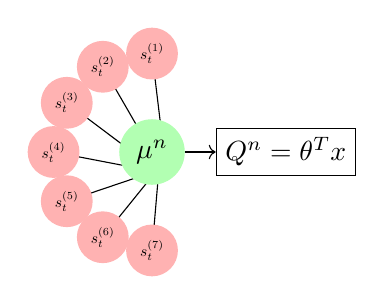
\begin{tikzpicture}
              \foreach \a in {1,2,...,7}{
              \path[draw, ->] (\a*360/6: 0.25cm)  -- (\a*360/12 + 60: 1.5cm-0.25cm) node[circle, fill=red!30, scale=0.8] {$\Scale[0.7]{s_t^{(\a)}}$};
              }
            \node[circle, style=dashed, fill=green!30] (A) {$\mu^n$};
            \node[rectangle] at (1.7,0) [draw] (B) {$Q^n = \theta^Tx$};
            \draw[->] (A) edge (B);
          \end{tikzpicture}
          \end{centering}
          \caption{A linear critic for $\mu^n$ }
      \end{figure}

      \end{column}
    \end{columns}

\end{frame}

\section{Results}
\begin{frame}
\frametitle{Results}
      \begin{columns}
      \begin{column}{0.6\textwidth}

  \textbf{The Training Regime}
  \begin{enumerate}
  \item We can train every neuron \textbf{simultaneously} without BP.
  \item There is no "extra" $Q$ network, just $2n$ parameters!
  \item Could be biologically plausible (certainly more reasonable than BP)
  \item Linear critic $\iff$ \emph{compatability} $\iff$ no bias in $Q^n$
  \end{enumerate}
      \end{column}
      \begin{column}{0.4\textwidth}
      \begin{figure}
          \begin{centering}
            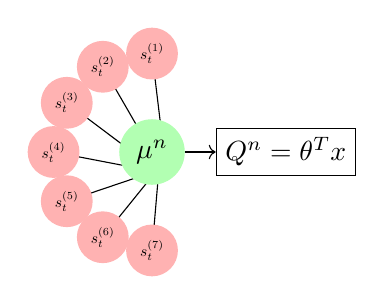
\begin{tikzpicture}
              \foreach \a in {1,2,...,7}{
              \path[draw, ->] (\a*360/6: 0.25cm)  -- (\a*360/12 + 60: 1.5cm-0.25cm) node[circle, fill=red!30, scale=0.8] {$\Scale[0.7]{s_t^{(\a)}}$};
              }
            \node[circle, style=dashed, fill=green!30] (A) {$\mu^n$};
            \node[rectangle] at (1.7,0) [draw] (B) {$Q^n = \theta^Tx$};
            \draw[->] (A) edge (B);
          \end{tikzpicture}
          \end{centering}
          \caption{A linear critic for $\mu^n$ }
      \end{figure}

      \end{column}
    \end{columns}

\end{frame}

\begin{frame}
  \frametitle{Experiments}
  \textbf{Experiment 1.}
  \begin{enumerate}
    \item Test if training $\mu$ with the full $Q^n$ $\implies$ each $\mu^n$ acting optimal to $Q^n$
    \item Is it true in practice that $\nabla_{W^{(n)}} Q^{n}(\mu^n) = \left(\nabla_{W} Q^\mu(\mu)\right)^{(n)}$?
  \end{enumerate}
    \textbf{Experiment 2.}
    \begin{enumerate}
      \item Train $\mu^n$ using $Q^n$ $\implies$ $Q$ optimal?
    \end{enumerate}
        \textbf{Experiment 3.}
    \begin{enumerate}
      \item Beat the state of the art in Atari 2600 environments!
    \end{enumerate}
\end{frame}
\begin{frame}
    \frametitle{Theorem 1}
    \begin{theorem}[Neurocomputational Decompostion]\label{thm:ncomp}
      Let $E$ be an environment and $\scriptn$ be a neurocomputational agent. Then there exists a set of agent environment pairs $\mathfrak{D}_\scriptn \defeq \{(E^n, \mu^n)\}_{n\in \scriptn}$ such that for every $n \in \scriptn$, the following diagram commutes
        \begin{equation}\label{eq:sub_env_com}
            \begin{tikzcd} %THe diagram for Q function decomposition.
  %-------------------------------------------------------------------------------------%
          \scriptv  \times \scripts \arrow{r}{\mu\circ\pi_2}
               \arrow{d}
                 {\pi_1  \times\epsilon \circ \pi_2}  &[+25pt]  \scripta    \\
  %-------------------------------------------------------------------------------------%%
            \overbrace{\scriptv \times \scriptv}^{(v_{t},\epsilon(s_t))}
                        \arrow{r}{D}
                                    \arrow[pos = 0.7]{rd}[swap]{\mu^n\circ\pi_1 + \pi_n \circ \pi_2}
                        & \overbrace{\scriptv}^{v_{t+1}}
                                              \arrow[two heads, pos=0.8]
                                                {d}
                                                {\pi_n}
                                              \arrow{u}{\delta} \\
  %%%%%%%%%%%%%%%%%%%%%%%%%%%%%%%%%%%%%%%%%%%%%%%%%%%%%%%%%%%%%%%%%%%%%%%%%%%%%%%%%%%%%%%
    &\reals
           \end{tikzcd}
        \end{equation}
    \end{theorem}
\end{frame}

\begin{frame}
    \frametitle{Theorem 2}
    \begin{theorem}
        If $\scriptn$ is a nuerocomputational agent in $E$, then policy gradient for $\mu$ agrees with the simultaneous policy gradients of its decomposition; that is for every $(E^n, \mu^n) \in \mathfrak{D}_\scriptn$
        \begin{equation}
            \nabla_{K^n} Q^{\mu^n}(v,\alpha)\Big|_{v=v_t,\alpha=\mu^n(v_t)} =\nabla_{K^n} Q^{\mu}(s,a)\Big|_{s=s_t,a=\mu(s_t)}
        \end{equation}
        for every time step $t$, where $K^n$ is the nth column of the linear voltage graph transition matrix, i.e. the weights of the connections from all neurons to neuron $n.$
    \end{theorem}
\end{frame}
\begin{frame}
    \frametitle{Experiment 1}
    % \textbf{Experiment 1}
    Compare subcritic Q-values to Q-values of the critic.
\end{frame}
\begin{frame}
    \frametitle{Experiment 2}
\end{frame}
\begin{frame}
    \frametitle{Experiment 2}
    \textbf{Goal:} Use the subcritics to train the actor network
    Progress: currently tweaking experiment.
\end{frame}
%------------------------------------------------

\begin{frame}
\Huge{\centerline{Questions?}}
\Small\centerline{wguss@berkeley.edu}
\end{frame}

%----------------------------------------------------------------------------------------

\end{document}
